
\documentclass[a4paper,11pt]{article}%,twocolumn
%% packages

\usepackage{blindtext} % needed for creating dummy text passages
%\usepackage{ngerman} % needed for German default language
\usepackage{amsmath} % needed for command eqref
\usepackage{amssymb} % needed for math fonts
\usepackage[colorlinks=true,breaklinks]{hyperref} % needed for creating hyperlinks in the document, the option colorlinks=true gets rid of the awful boxes, breaklinks breaks lonkg links (list of figures), and ngerman sets everything for german as default hyperlinks language
\usepackage[hyphenbreaks]{breakurl} % ben�tigt f�r das Brechen von URLs in Literaturreferenzen, hyphenbreaks auch bei links, die �ber eine Seite gehen (mit hyphenation).
\usepackage{xcolor}
\definecolor{c1}{rgb}{0,0,1} % blue
\definecolor{c2}{rgb}{0,0.3,0.9} % light blue
\definecolor{c3}{rgb}{0.3,0,0.9} % red blue
\hypersetup{
    linkcolor={c1}, % internal links
    citecolor={c2}, % citations
    urlcolor={c3} % external links/urls
}
%\usepackage{cite} % needed for cite
\usepackage[square,authoryear]{natbib} % needed for cite and abbrvnat bibliography style
\usepackage[nottoc]{tocbibind} % needed for displaying bibliography and other in the table of contents
\usepackage{graphicx} % needed for \includegraphics 
\usepackage{longtable} % needed for long tables over pages
\usepackage{bigstrut} % needed for the command \bigstrut
\usepackage{enumerate} % needed for some options in enumerate
%\usepackage{todonotes} % needed for todos
\usepackage{makeidx} % needed for creating an index
\makeindex
\usepackage{gensymb}
\usepackage{url}
\usepackage{psfrag}
\usepackage{multirow}
\usepackage{subfigure}
%% page settings

\usepackage[top=20mm, bottom=20mm,left=15mm,right=15mm]{geometry} % needed for page border settings
\parindent=0mm % for space of first line of new text block
\sloppy % for writing with hyphenless justification (tries to)
\hyphenation{} % use hyphenation of tolerance parametershttp://www.jr-x.de/publikationen/latex/tipps/zeilenumbruch.html
\hyphenpenalty=10000
\exhyphenpenalty=10000
\usepackage{fancyhdr} % needed for head and foot options
%% my macros

%% Text fomats
\newcommand{\tbi}[1]{\textbf{\textit{#1}}}

%% Math fonts
\newcommand{\bbA}{\mathbb{A}}
\newcommand{\bbB}{\mathbb{B}}
\newcommand{\bbC}{\mathbb{C}}
\newcommand{\bbD}{\mathbb{D}}
\newcommand{\bbE}{\mathbb{E}}
\newcommand{\bbF}{\mathbb{F}}
\newcommand{\bbG}{\mathbb{G}}
\newcommand{\bbH}{\mathbb{H}}
\newcommand{\bbI}{\mathbb{I}}
\newcommand{\bbJ}{\mathbb{J}}
\newcommand{\bbK}{\mathbb{K}}
\newcommand{\bbL}{\mathbb{L}}
\newcommand{\bbM}{\mathbb{M}}
\newcommand{\bbN}{\mathbb{N}}
\newcommand{\bbO}{\mathbb{O}}
\newcommand{\bbP}{\mathbb{P}}
\newcommand{\bbQ}{\mathbb{Q}}
\newcommand{\bbR}{\mathbb{R}}
\newcommand{\bbS}{\mathbb{S}}
\newcommand{\bbT}{\mathbb{T}}
\newcommand{\bbU}{\mathbb{U}}
\newcommand{\bbV}{\mathbb{V}}
\newcommand{\bbW}{\mathbb{W}}
\newcommand{\bbX}{\mathbb{X}}
\newcommand{\bbY}{\mathbb{Y}}
\newcommand{\bbZ}{\mathbb{Z}}
\usepackage[ framed, numbered]{matlab-prettifier}%framed,%
\usepackage{listings}
\usepackage{physics}
\usepackage{pdfpages}
\usepackage[toc,page]{appendix}
\usepackage{float}
\usepackage{pifont}


\begin{document}
\begin{titlepage}
\center % Center everything on the page

%-------------------------------------------------------------------------------------
%	HEADING SECTIONS
%------------------------------------------------------------------------------------
\textbf{\large Department of Electrical and Computer Engineering}\\[0.5cm]
\textbf{\Large University of Colorado at Boulder}\\[1cm]
\textbf{\large ECEN5730 - Practical PCB design}\\[2cm]

\includegraphics[width=0.3\textwidth]{figures/cu}\\[2cm] 

	
%-------------------------------------------------------------------------------------
%	TITLE SECTION
%------------------------------------------------------------------------------------

\textbf{\Huge Board Good Layout/Bad Layout }\\[0.2cm]

\textbf{\Large Report}\\[2cm]
\vspace{1.5cm}
\begin{figure}[H]
	\centering
	
\includegraphics[scale=0.2]{figures/qr_download.png}
	\label{555_schematic}
\end{figure}\vspace{1.5cm}


%----------------------------------------------------------------------------------------
%	MEMBERS SECTION
%----------------------------------------------------------------------------------------


\vfill

\textbf{\large Submitted by}

{\large Parth Thakkar}\\[0.5cm]




%----------------------------------------------------------------------------------------
%	DATE SECTION
%----------------------------------------------------------------------------------------

\textbf{\large Submitted on}\\
\textbf{\Large \today} % Date, change the \today to a set date if you want to be precise

%----------------------------------------------------------------------------------------

\vfill % Fill the rest of the page with whitespace

\end{titlepage}

\pagebreak

\tableofcontents
\listoffigures
\listoftables
\vfill
\begin{center}
	\textbf{\textit{*PDF is clickable}}
\end{center}

\pagebreak

\section{Introduction}

In this project, I aimed to build and examine a circuit featuring a 555 timer set up as an astable multivibrator that operates slowly. I added a potentiometer to the circuit to control the duty cycle, targeting a 50\% duty cycle at a frequency of 500Hz, with the flexibility to adjust it from roughly 10\% to 90\%.\\

\textbf{Measurements to be Conducted:}

\begin{enumerate}
	\item \textbf{Voltage Measurement:} Check the voltage at the output pin of the 555 timer both without any load and then with a 1k resistor connected. This will help determine the Thevenin resistance of the circuit, which is a way to simplify the network seen by the load.
	\item \textbf{Oscilloscope Analysis:} Use an oscilloscope equipped with a 10x probe to observe the rise and fall times of the 555 timer's output signal. This equipment will also be used to verify the frequency and duty cycle of the output, ensuring that the circuit operates as intended.
	\item \textbf{Noise Measurement:} Examine the switching noise present on the power rail. Switching noise, or ripple, can affect the performance of the circuit and is especially important in sensitive applications.
\end{enumerate}

For the construction, 1206 size surface-mount device (SMD) components were chosen and soldered onto a printed circuit board (PCB). This choice of components and the assembly process highlight the practical aspects of PCB design flow, from selecting appropriate parts to the actual soldering and testing of the finished board.

\section{Project Plan}
\begin{enumerate}
	\item Incorporate an external 5V AC to DC adapter for board power.
	Utilize a slow 555 Timer Integrated Circuit (IC).
	\item Design the timer circuit to target approximately 500 Hz frequency and 50\% duty cycle.
	\item Include a decoupling capacitor with the 555 IC to minimize switching noise.
	\item Implement a copper-poured ground plane.
	\item Install 4 LEDs of identical color with series resistors valued at 10k, 1k, 300, and 50 Ohms.
	\item Add indicator lights, testing points, and isolation switches for enhanced functionality and diagnostics.
\end{enumerate}



\section{Risk Management}
\begin{enumerate}
	\item Test points will be strategically placed and clearly labeled for easy identification.
	\item Isolation switches will be installed at each stage to facilitate troubleshooting and debugging.
	\item The 555-timer will be chosen based on the required output current to ensure proper operation.
	\item Signal lines will have a width of 6 mils to maintain signal integrity.
	\item Power lines will be designed with a width of 20 mils to distinguish them easily and support adequate current flow.
	\item The potentiometer will be oriented correctly to ensure proper adjustment of the circuit. and checking hole size and distance of the through holes for potentiometer
	\item The diode will be oriented correctly to ensure correct current flow direction. and checking hole size and distance of the through holes for diode
	\item The output from Altium Designer will be checked for feasibility, with Gerber files generated accurately for manufacturing.
	\item The schematic will be compared with the breadboard implementation to ensure the design works as intended in a practical setting.
	
\end{enumerate}

\section{Block Diagram, Schematic and Layout}
\subsection{Block Diagram Description}
The block diagram for the 555 timer PCB project is divided into three main sections:

\begin{enumerate}
	\item Power Supply: This section includes the external 5V AC to DC charger input, ensuring the board receives a stable power supply. It is isolated from the rest of the circuit to prevent noise interference.
	\item 555 Timer Circuit: The core of the project, where the 555 timer IC operates in an astable mode to generate a variable frequency output. This section is designed to allow adjustments in the duty cycle through a potentiometer and is isolated for easy modification or debugging.
	\item Output Unit: Includes the output stage where the signal from the 555 timer is utilized. This could involve LEDs, a speaker, or other components to demonstrate the output signal's behavior. Isolation switches are also present here to detach the unit when necessary.
\end{enumerate}

\begin{figure}[H]
	\centering
	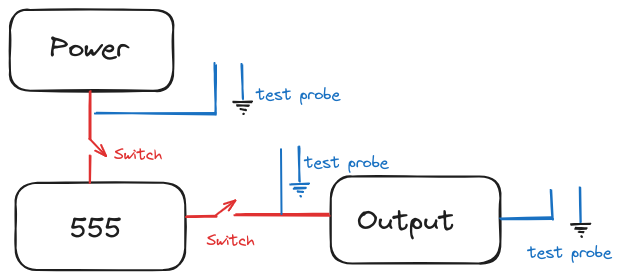
\includegraphics[scale=0.4]{figures/ne555_blockdiagram}
	\caption{Block diagram}
\end{figure}

\subsection{Component listings}
\begin{table}[H]
	\centering 
	\begin{tabular}{l c c c c}
		\hline
		\textbf{Component Name}&\textbf{Usecase}&\textbf{Symbol}&\textbf{Value}&\textbf{Was in inventory}\\\hline
		&&\\
1 x Capacitor&Charging Discharging Capacitor&C5&0.1$\mu$F&\ding{55}\\
1 x Potentiometer&Change the Waveform Dutycycle&R2&10k$\ohm$&\ding{55}\\
1 x Diode&Discharging bypass Diode&D1&&\ding{55}\\
1 x Resistor&Discharging rate Resistor&R3&15k$\ohm$&\ding{55}\\
1 x Capacitor&Decoupling cap&C5&22$\mu$F&\ding{51}\\
1 x Capacitor&Filter Capacitor&C5&10$\mu$F&\ding{51}\\
1 x Resistor&Current Limiting resistor&R4&50$\ohm$&\ding{51}\\
1 x Resistor&Current Limiting resistor&R5&300$\ohm$&\ding{51}\\
1 x Resistor&Current Limiting resistor&R6&1k$\ohm$&\ding{51}\\
1 x Resistor&Current Limiting resistor&R7&10k$\ohm$&\ding{51}\\
1x NE555&Timer IC&U1&&\ding{51}\\
3 x Switch&To isolate the Circuit&SW&&\ding{51}\\
3 x LEDs&For output&LED&&\ding{51}\\
\hline\hline
	\end{tabular}
	\caption{Component list}
	\label{filterspecs}
\end{table}



\subsection{Schematic Overview}
The schematic includes key components like the 555 timer IC, a diode, and a potentiometer to achieve a variable duty cycle. The diode is strategically placed to have negligible forward resistance, allowing current to flow in one direction during the capacitor charging phase. This design choice ensures that the diode does not interfere with the charging process, while the potentiometer allows for adjustment of the duty cycle.

\begin{figure}[H]
	\centering
	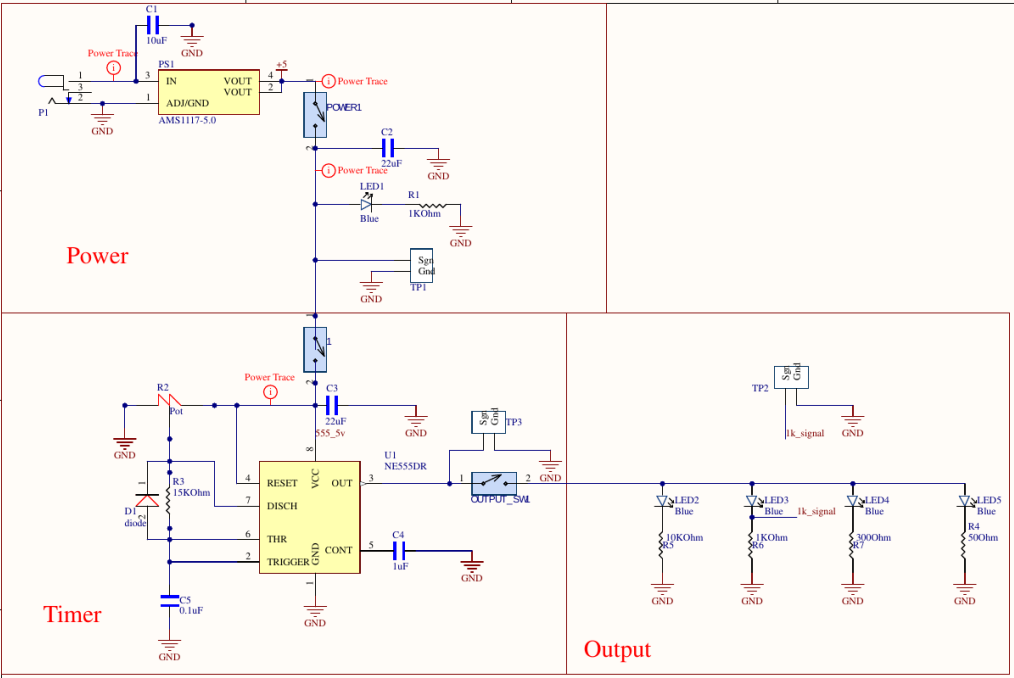
\includegraphics[scale=0.4]{figures/overall_sch.png}
	\caption{Schematic}
\end{figure}


\subsection{Layout Considerations}
For the PCB layout, several factors are critical:

\begin{enumerate}
	\item \textbf{Test Probes:} Designated points for measuring power rail voltage, the output from the 555 timer, and the voltage across a 1k resistor. Each test point is accessible via individual switches for isolation.
	\item \textbf{Decoupling Capacitor:} Positioned as close to the 555 timer IC as possible to minimize switching noise and stabilize the power supply to the IC.
	\item \textbf{Ground Pour:} Implementing a ground pour around signal and power traces to enhance signal integrity and provide a better return path for signals, reducing interference and improving circuit performance.
\end{enumerate}


\pagebreak
\section{Manufacturing and Assembly}

Breadboard Implementation:

\begin{figure}[H]
	\centering
	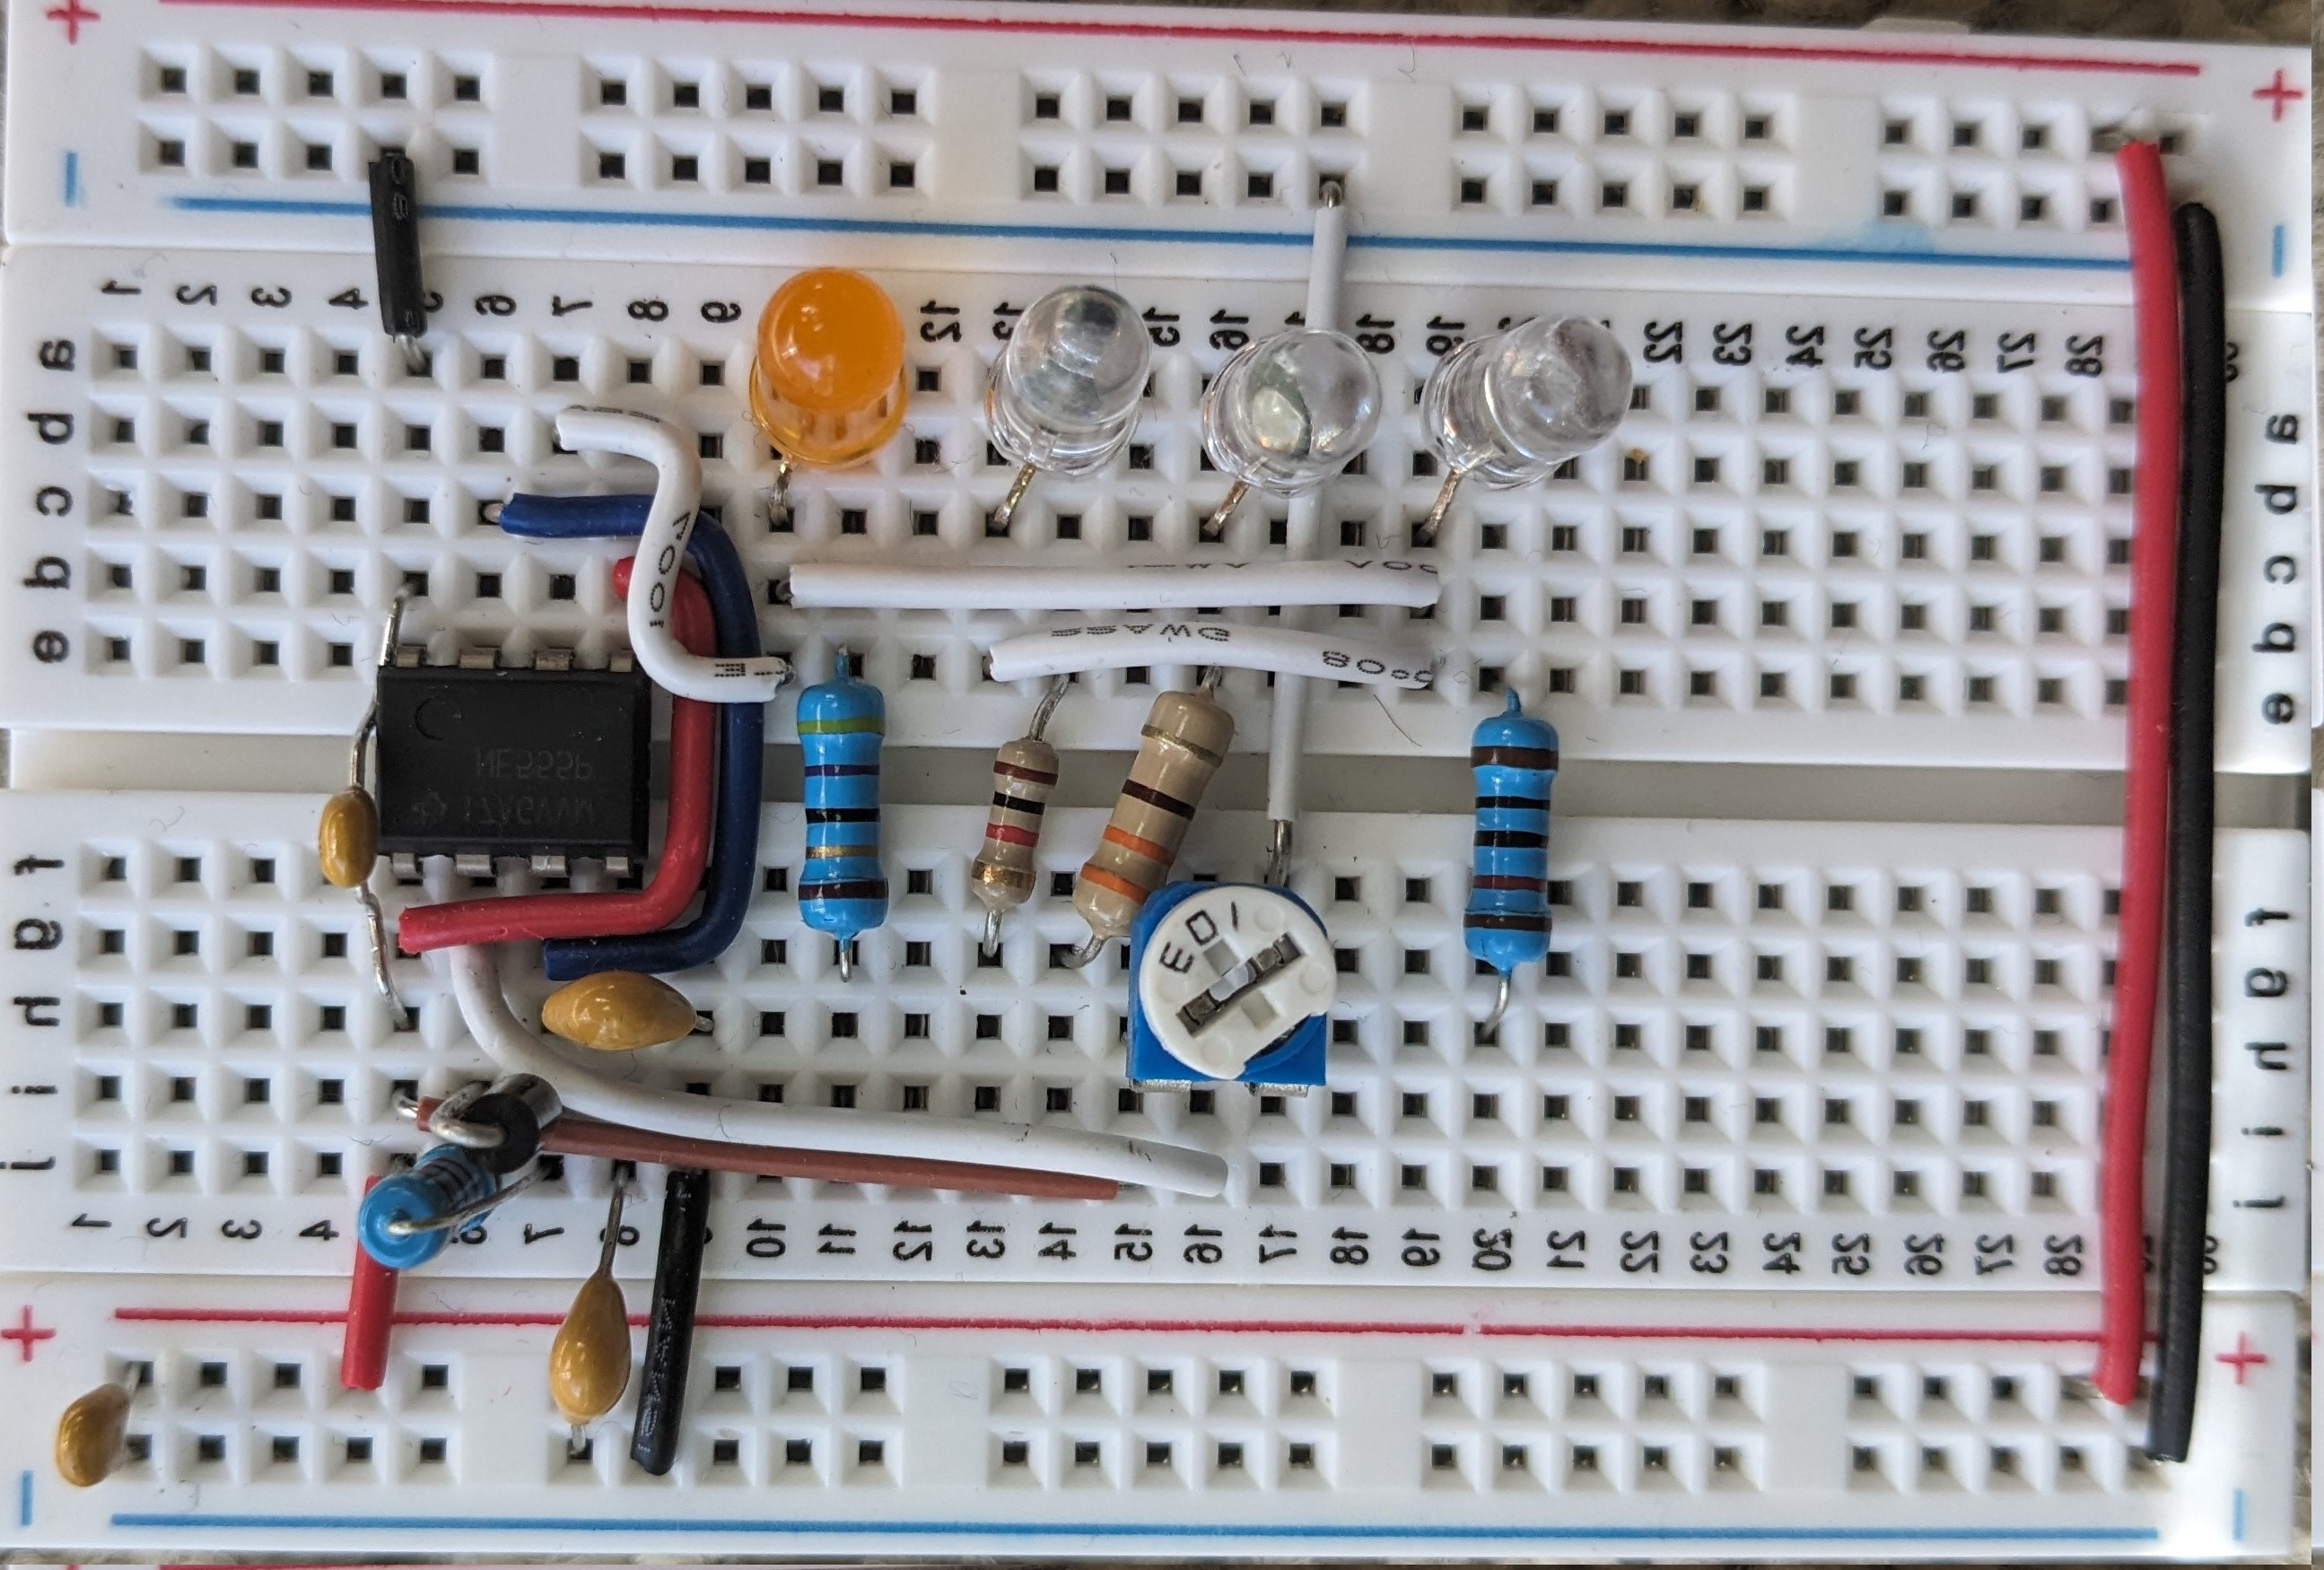
\includegraphics[scale=0.2]{figures/breadboard.jpg}
	\caption{Breadboard Implementation}
	\label{breadboard}
\end{figure}


The PCB design considerations mentioned should be followed during the manufacturing and assembly process to ensure the final product meets the intended specifications and performs as designed in practical applications.\\

Here is the PCB design for top layer and bottom layer:\\

\begin{figure}[H]
	\centering
	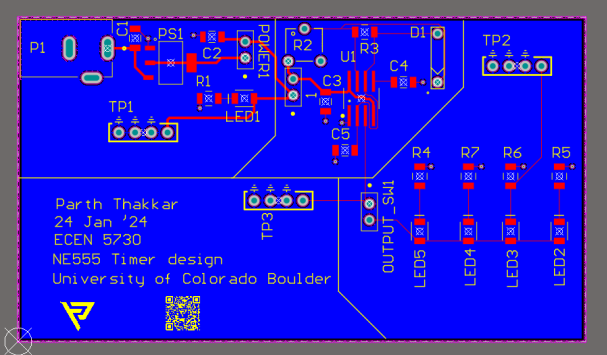
\includegraphics[scale=0.8]{figures/top.png}
	\caption{Top layer PCB}
	\label{top}
\end{figure}

\begin{figure}[H]
	\centering
	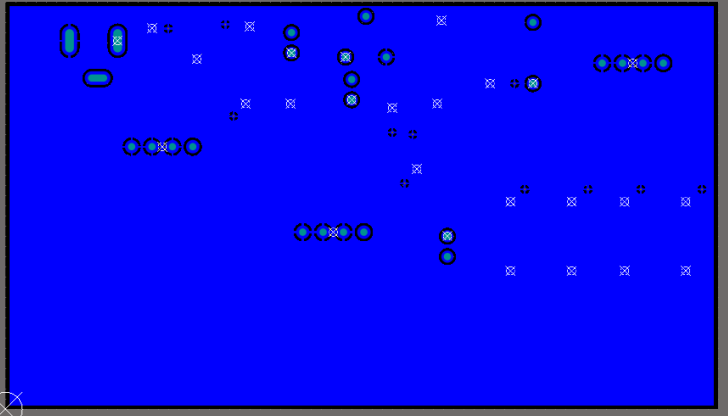
\includegraphics[scale=0.7]{figures/bottom.png}
	\caption{Bottom Layer PCB}
	\label{bottom}
\end{figure}

This is the photo of the PCB after manufacturing\\

\begin{figure}[H]
	\centering
	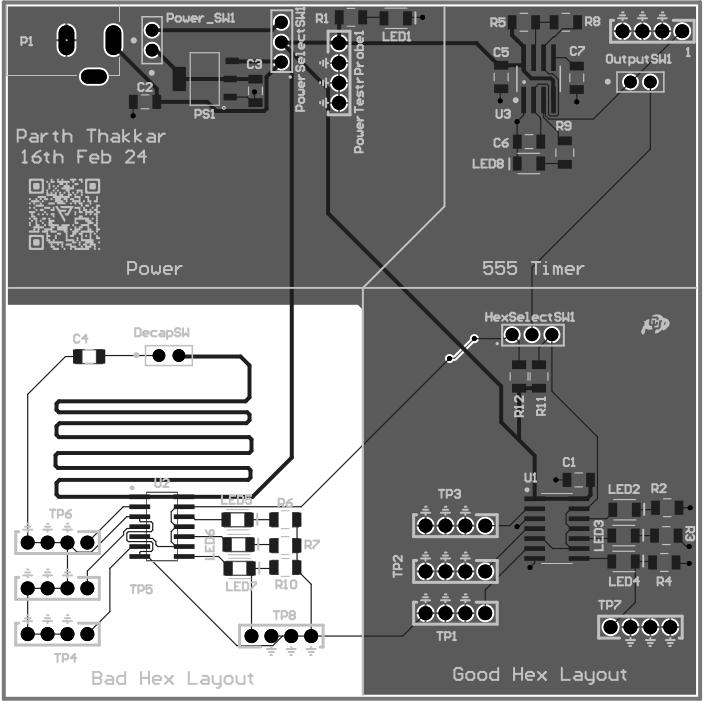
\includegraphics[scale=0.1]{figures/pcb.jpg}
	\caption{Manufactured PCB}
\end{figure}

\begin{figure}[H]
	\centering
	\includegraphics[scale=0.1]{figures/pcb_comp.jpg}
	\caption{PCB with components soldered}
\end{figure}


\begin{figure}[H]
	\centering
	\includegraphics[scale=0.1]{figures/pcb_comp_on.jpg}
	\caption{First time turning on the PCB}
\end{figure}



\section{Calculations for Duty Cycle and Frequency}


Circuit given in the lab manual can give us approx 60\% 
of duty cycle, So I have come up with my circuit to make the circuit work at 50\% duty cycle and also be able to vary the circuit\\

\begin{enumerate}
	\item for simple circuit we can see that the overall time for one cycle would be\\
	\begin{flalign*}
		& T_{total} = T_{charging} + T_{discharging}&& \\\\
		& \textbf{And expanding each timing term would give us,}&& \\
		&T_{charging} = 0.693 \cdot(R_1 + R_2) \cdot C&& \\
		& T_{discharging} = 0.693 \cdot(R_2) \cdot C&& \\\\
		&\textbf{so the total time for charging and Discharging would be, }&& \\
		&T_{total} = 0.693 \cdot(R_1 + R_2) \cdot C + 0.693 \cdot(R_2) \cdot C&& \\
		&T_{total} = 0.693 \cdot(R_1 +  2 \cdot R_2) \cdot C&& \\
	\end{flalign*}
	\item Modifications for 50\% Duty Cycle:\\
	By introducing a bypass diode across R2, R2
	  is effectively removed from the discharging equation, simplifying ,
	\begin{flalign*}
	&T_{charging} = 0.693 \cdot(R_1 + R_2) \cdot C&& \\
	&T_{discharging} = 0.693 \cdot C&& \\\\
	&T_{total} = 0.693 \cdot(R_1 + R_2) \cdot C&& \\
	\end{flalign*}

		
	Here is the schematic with bypass diode to reduce the time for discharging the cap
	\begin{figure}[H]
		\centering
		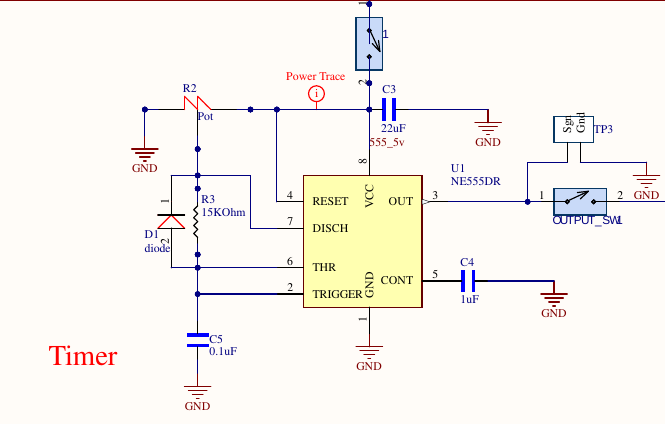
\includegraphics[scale=0.8]{figures/timer_sch}
		\caption{Schematic for variable duty-cycle 555 Timer}
		\label{555_schematic}
	\end{figure}

	Equation for schematic with bypass diode is,
	\begin{gather}
		T_{total} = 0.693 \cdot(2 \cdot R_1) \cdot C
	\end{gather}

	We need 50\% duty cycle so we will assume that $T_{charging}$ and $T_{discharging}$ is same.
	\begin{flalign*}
		& T_{charging} = T_{discharging}&& \\
		& 0.693 \cdot(R_1 + R_2) \cdot C = 0.693 \cdot C&& \\
		& R_1 = R_2 \textit{(negative sign implies Current in reverse direction)}
	\end{flalign*}

	We need 500Hz frequency and we are assuming C as 0.1$\mu$F putting this value in the equation and putting $R_1 = R_2$ 	
	\begin{flalign*}
		& T_{total} = 0.693 \cdot(R_1 + R_2) \cdot C && \\
		& \left(\frac{1}{500} \right) = 0.693 \cdot(R_1 + R_2) \cdot C && \\
		& \left( \frac{0.002}{0.693} \right) = 2 \cdot R_1 \cdot 0.1 \cdot 10^{-6} && \\
		& \boxed{R_1 = 15k\ohm} && \\
	\end{flalign*}

	So, I have added $R_2$ as 15k ohm and $R_1$ is variable Potentiometer of 10k$\ohm$ so that we can change the output frequency.

	\item Modification due to component not being available in inventory\\
	\textbf{\textit{Due to comonents not being in the inventory I had to change the values for the components. I used 1uF instead of 0.1uF and 1k instead of 15k, calculation for the components in below}}

	
	\begin{flalign*}
		&T_{total} = 0.693 \cdot(2 \cdot R_1) \cdot C &&\\
		&T_{total} = 0.693 \cdot(2 \cdot 1000 \ohm) \cdot 1 \cdot 10^{-6} &&\\
		&T_{total} = 1386 \cdot 10 \cdot 10^{-6} &&\\
		&T_{total} = 0.001386 Sec&&\\
		& \text{So output frequency would be,} &&\\
		&f_{total} = 721.5 Hz &&\\
	\end{flalign*}

	\textbf{\textit{Which you will see is matching with the actual output freqency of the board}}
	
\end{enumerate}

\section{Output Waveforms}

Below Schematic \ref{cap} shows charging discharging of capactor at constant rate, it shows that it will start charging at 1/3 V and start discharging at 2/3 V .

As the capacitor charges up to 2/3 of (VDD) and discharges to 1/3 of VDD, the output voltage of the 555 timers will be about 2 V less than VDD. Voltage loss is impacted by even load voltage decline.
\begin{figure}[H]
	\centering
	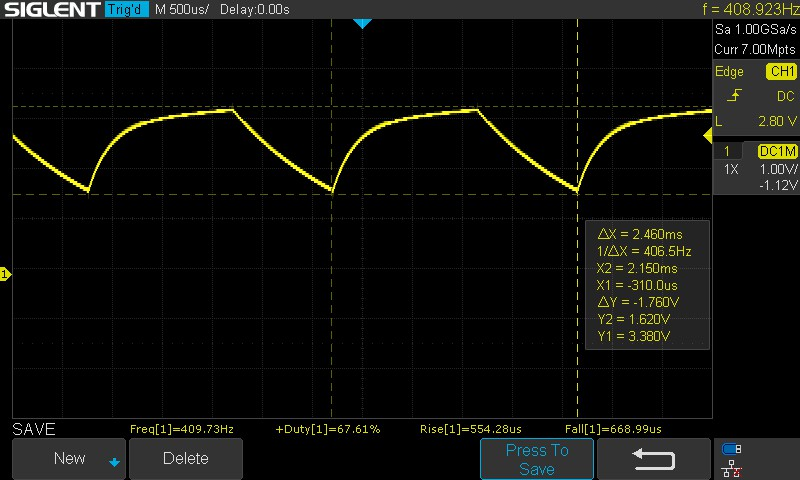
\includegraphics[scale=0.5]{figures/cap}
	\caption{Capacitor Charging and Discharging}
	\label{cap}
\end{figure}


We can see the power rail noise in the circuit and it is around 70mV, which is feasible.(with load connected)
\subsection{Power Rail noise}
\begin{figure}[H]
	\centering
	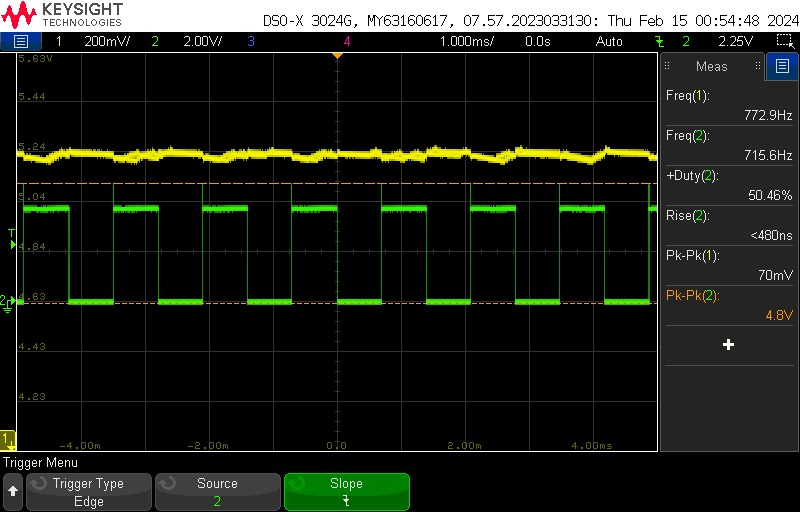
\includegraphics[scale=0.6]{figures/power_noise_overall.jpg}
	\caption{Power Rail noise with Load connected}
	\label{cap}
\end{figure}



\subsection{Output without Load}


\subsubsection{555 with no Load}
555 output without connecting the load, causes 40mV peak to peak on power rail. with same duty cycle and same frequency.
\begin{figure}[H]
	\centering
	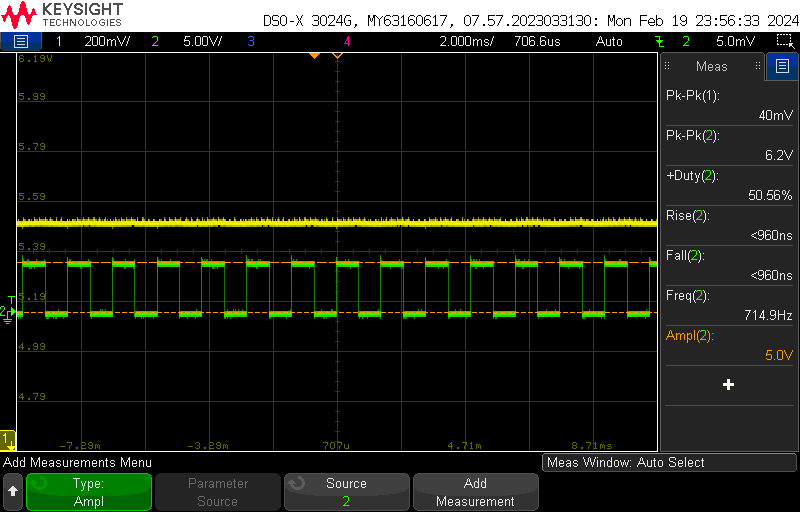
\includegraphics[scale=0.5]{figures/without_load.png}
	\caption{Power Rail noise without Load connected}
\end{figure}


\subsubsection{555 Rise time with no Load}
Rise time for resistive load is not being connected, it is around 84nS.
\begin{figure}[H]
	\centering
	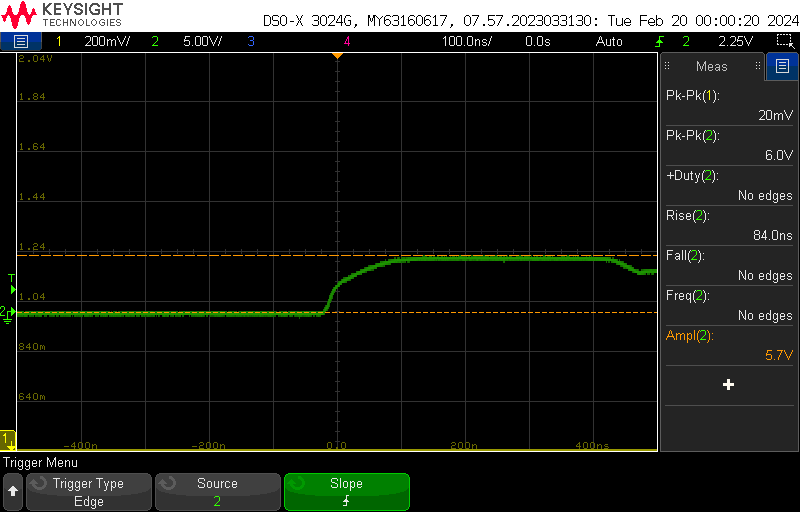
\includegraphics[scale=0.5]{figures/rise_without_load.png}
	\caption{Rise time without load}
\end{figure}


\subsubsection{555 Fall time with no Load}
Fall time without connecting load is around 12.4nS.
\begin{figure}[H]
	\centering
	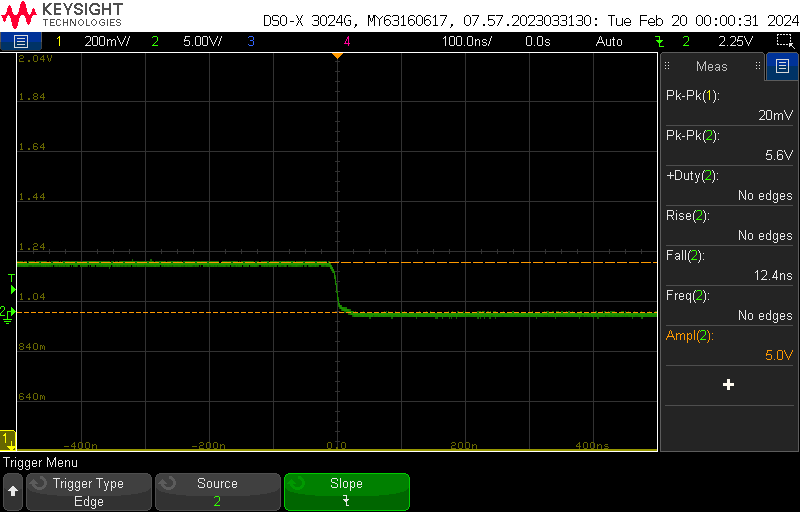
\includegraphics[scale=0.5]{figures/fall_without_load.png}
	\caption{Fall time without load}
\end{figure}



\subsection{Output with Load}



\subsubsection{555 with Load}
Overall noise on 5v rail due to switching with load is around 80mV peak to peak
\begin{figure}[H]
	\centering
	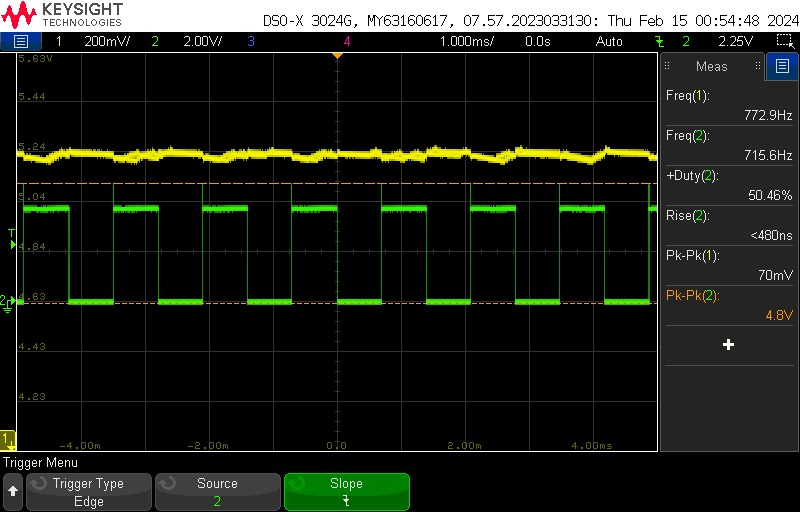
\includegraphics[scale=0.6]{figures/power_noise_overall.jpg}
	\caption{555 output with all the load connected}
\end{figure}


\subsubsection{555 Rise time with Load}
Rise time for resistive load being connected, it is around 82nS.
\begin{figure}[H]
	\centering
	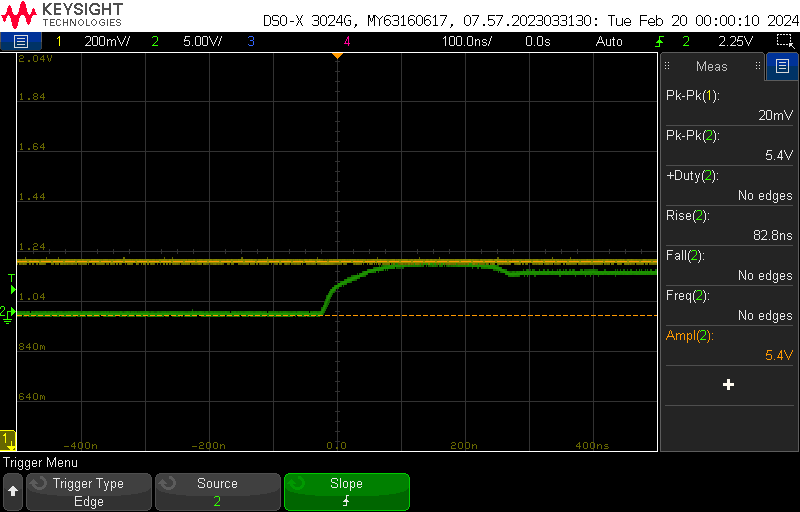
\includegraphics[scale=0.6]{figures/rise_w_load.png}
	\caption{Rise time with load connected}
\end{figure}

\subsubsection{555 Fall time with Load}
Fall time with connecting load is around 75.2nS.
\begin{figure}[H]
	\centering
	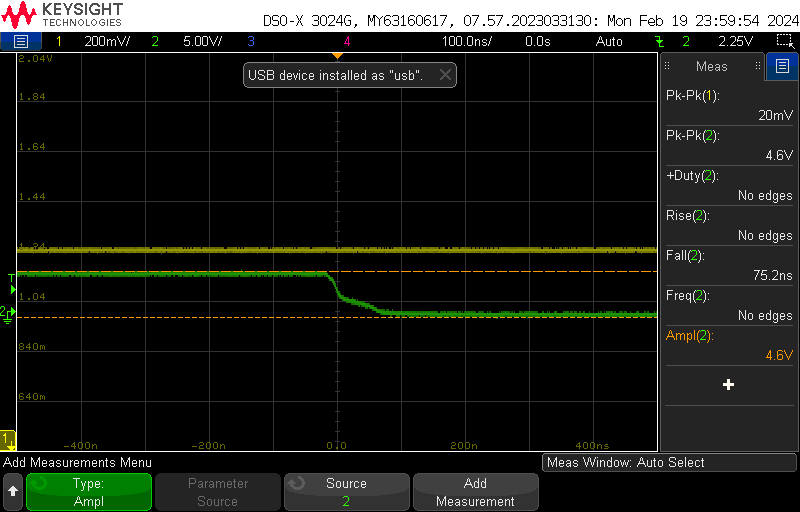
\includegraphics[scale=0.6]{figures/fall_w_load.png}
	\caption{Fall time with load connected}
\end{figure}



\section{Calculating Thevenin resistance for 555}

With Independent Sources: Temporarily remove the load resistance (if any) from the circuit. Replace all voltage sources with short circuits and all current sources with open circuits. The resistance seen across the terminals is the Thevenin resistance $R_{th}$.

	\textbf{Isolation of Circuit:} Initially, the load resistance 1k$\ohm$ is removed to isolate the circuit. We can do that by removing switch for output. This step is to calculate the inherent resistance of the circuit.


	\begin{table}[H]
		\centering
	
		\begin{tabular}{c c}
	
			\textbf{Voltage Without Load Resistance}&\textbf{Voltage With Load Resistance}\\
			
			5.0V&4.0V\\\vspace{0.5cm}

		\end{tabular}
		\caption{voltage with and without load resistance}
		\label{voltagewithandwithoutresistance}
	\end{table}

	\textbf{Voltage Measurements:}
		Without Load Resistance: The open-circuit voltage Voc
  is measured across the terminals, which is equivalent to the Thevenin voltage Vth

		With Load Resistance: The circuit voltage Vload
  is measured again after reintroducing the load resistance of 1k$\ohm$.

	\begin{flalign*}
	\label{equation_th}
	R_{th} = R_{load}\left(\frac{V_{th} - V_{load}}{V_{load}} \right)
	\end{flalign*}

	\pagebreak

	So first we will measure voltage without load resistance

	\begin{figure}[H]
		\centering
		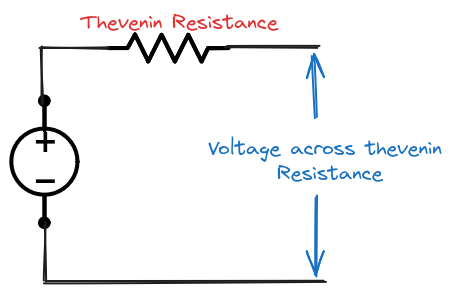
\includegraphics[scale=0.6]{figures/open_th.png}
		\caption{Voltage measurement without load resistance}
	\end{figure}

	We got around 5V of voltage in without load Resistance $R_{load}$.

	Now we will measure Thevenin voltage with load resistance $R_{load}$ of 300$\ohm$.
	
	\begin{figure}[H]
		\centering
		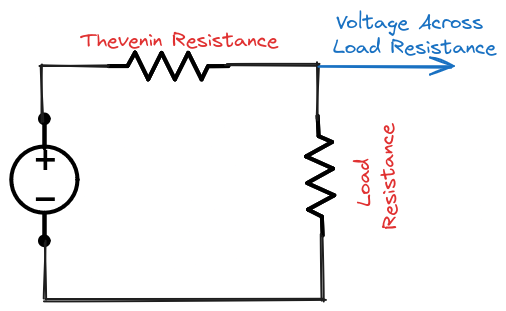
\includegraphics[scale=0.6]{figures/th.png}
		\caption{Voltage drop due to load resistance}
	\end{figure}

	This time, We got around voltage drop of 0.680V across the load resistance of 300$\ohm$.

	and putting values in the equation \ref{equation_th} will give us,

	\begin{flalign*}
		&R_{th} = 300 \left(\frac{5 - 4}{4} \right)&&\\
		&R_{th} = 300 \cdot 0.25&&\\
		&\boxed{R_{th} = 75\ohm}\\
	\end{flalign*}
	

	So conclusion is that the $R_{th}$ of power supply would be around 75$\ohm$.


\section{What worked ?}

\begin{table}[H]
	\centering

	\begin{tabular}{l c}

		\textbf{Parameter}&\textbf{Worked ?}\\\hline
		5V Input&\ding{51}\\
		Desired frequency of Output&\ding{51}\\
		Duty cycle as calculated&\ding{51}\\
		Low switching noise&\ding{51}\\
		Current across LEDs&\ding{51}\\

	\end{tabular}
	\caption{Rise-time and Fall-time}
	\label{tab_rise_fall}
\end{table}

\section{Mistakes Made}

\textbf{Overview of Mistakes and Adjustments}
\begin{enumerate}
	\item \textbf{Component Availability Issue:} You planned to use a 0.1uF capacitor and a 15k resistor in your circuit design, aiming for a target frequency of 500Hz based on your calculations.
	\item \textbf{Substitution Required:} Due to the lack of the specified components in the lab inventory, you had to use a 1uF capacitor and a 1k resistor instead.
	\item \textbf{Outcome:} This substitution led to achieving a frequency of 700Hz in the actual circuit, deviating from the calculated target of 500Hz.
	\item \textbf{Breadboard Confirmation:} Despite this discrepancy in the PCB implementation, you were able to achieve the intended 500Hz frequency on a breadboard setup, confirming the accuracy of your original calculations and design intentions.
\end{enumerate}

\textbf{Analysis}

\textbf{Impact of Component Variations:} This situation illustrates how variations in component values can significantly affect the performance of electronic circuits, especially in timing-critical applications like those involving the 555 timer.


Other than that, no hard or soft errors on the board.

\section{Learnings}

The lab demonstrated the characteristics of 555 timer ICs in various configurations(555 timer circuit set up as an astable multivibrator). The primary objectives were met. And creating 2 layer PCB with understanding of how to use altium, debug the PCB and use theoretical knowledge to create it in software and implement in PCB.\\

Here are the key lessons learned:\\

\begin{enumerate}
	\item \textbf{Circuit Design and Simulation}\\
	Planning and simulating the circuit before building it is crucial. Adjusting the 555 timer's duty cycle to hit a specific frequency and duty cycle showed how selecting the right components matters.
	\item \textbf{Noise Management}\\
	The project highlighted how electronic circuits can have noise issues. Using a decoupling capacitor and a well-designed ground plane helped reduce noise.
	\item \textbf{Risk Management and Troubleshooting}\\
	Labeling test points and using switches help find and fix problems faster.
	Planning ahead makes solving issues easier.
	\item \textbf{Component Selection and Adaptability}\\
	Sometimes, you need to change parts because the ones you planned to use aren't available. This teaches you to be flexible.
	Being able to adjust keeps your project moving forward.
	\item 
	\textbf{Theoretical vs. Practical Differences}\\
	Tests show that what you calculate might not always match what actually happens. This means you might need to try different things to get your design right.
	Learning from what doesn't work as expected is important. It helps you make your design better.
	
\end{enumerate}





\vfill
\hrule
\vspace{0.5cm}



\vspace{1cm}
\hrule
\vspace{0.5cm}


%---------------------------------------------------------------------------
\end{document}
-
